\chapter{All Regional Fits}
\label{appendix:curvefits}

For space reasons, we did not include model fits for all of the potential regions in figure \ref{fig:curves}. Here, we provide full figures for all of the HHS regions (see fig \ref{fig:hhs_curves_all}) and both of the counties that provided disease data to compare against (see fig \ref{fig:local_curves_all}).

\begin{figure}
\centering
\begin{subfigure}[b]{0.49\textwidth}
	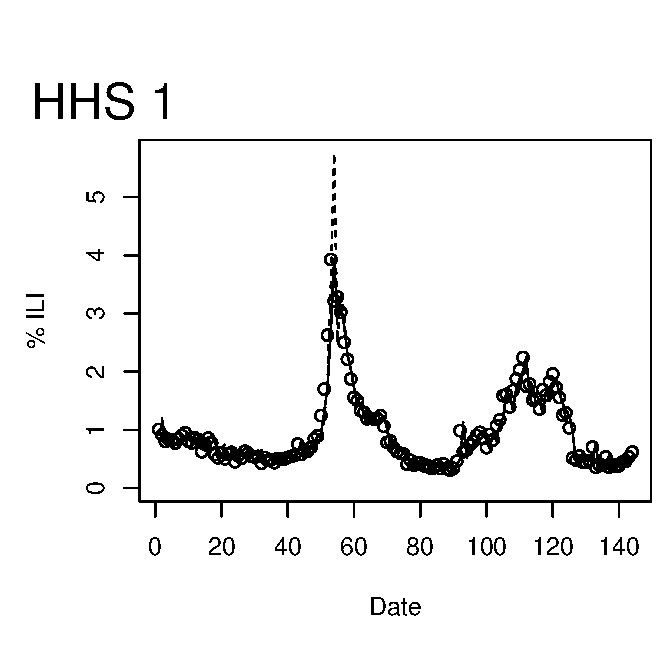
\includegraphics[width=\textwidth]{longitude/figs/nowcastHHS_1.eps}
\end{subfigure}
\begin{subfigure}[b]{0.49\textwidth}
	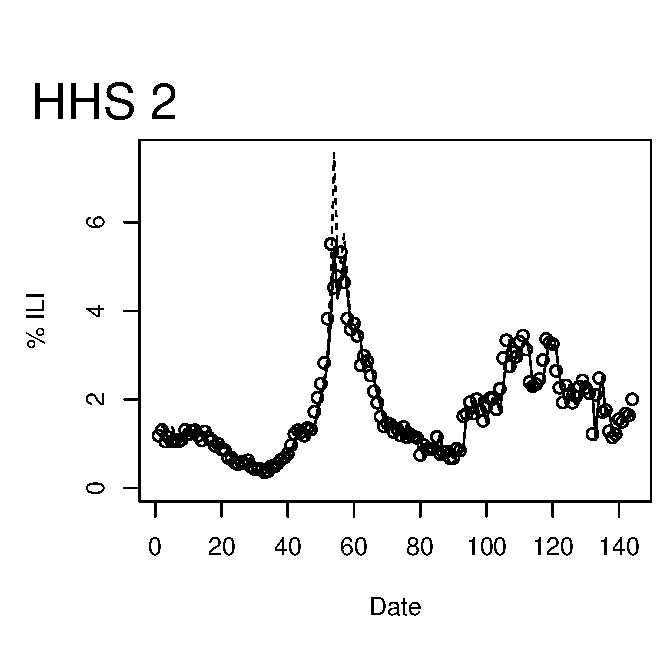
\includegraphics[width=\textwidth]{longitude/figs/nowcastHHS_2.eps}
\end{subfigure}
\\
\begin{subfigure}[b]{0.49\textwidth}
	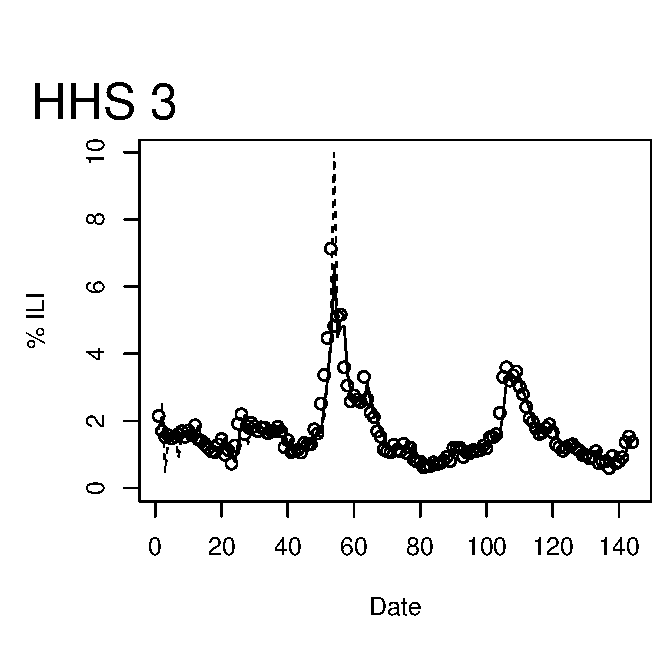
\includegraphics[width=\textwidth]{longitude/figs/nowcastHHS_3.eps}
\end{subfigure}
\begin{subfigure}[b]{0.49\textwidth}
	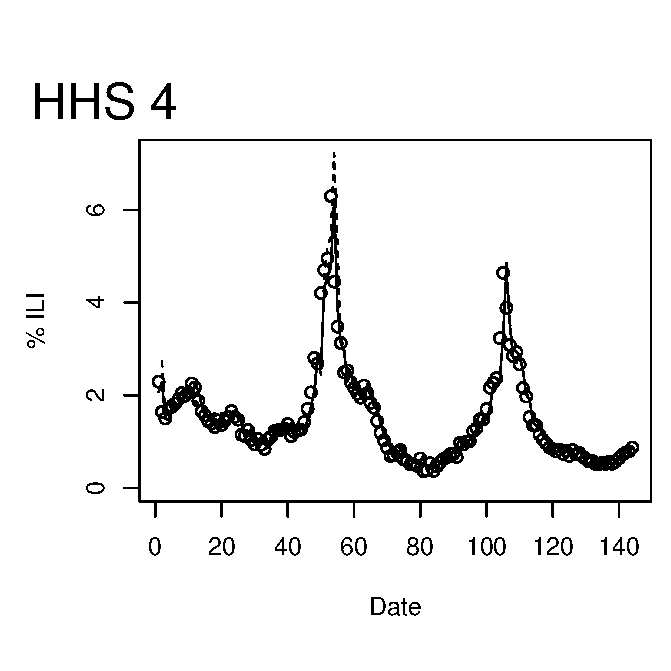
\includegraphics[width=\textwidth]{longitude/figs/nowcastHHS_4.eps}
\end{subfigure}
\\
\begin{subfigure}[b]{0.49\textwidth}
	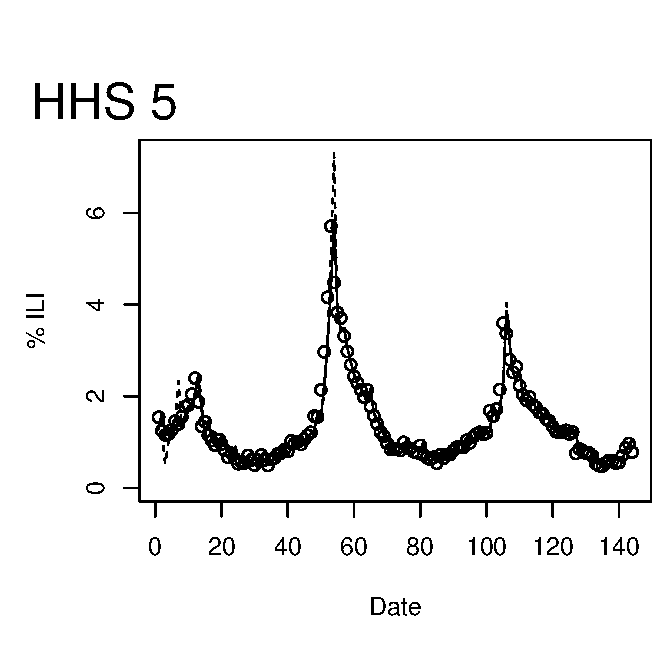
\includegraphics[width=\textwidth]{longitude/figs/nowcastHHS_5.eps}
\end{subfigure}
\begin{subfigure}[b]{0.49\textwidth}
	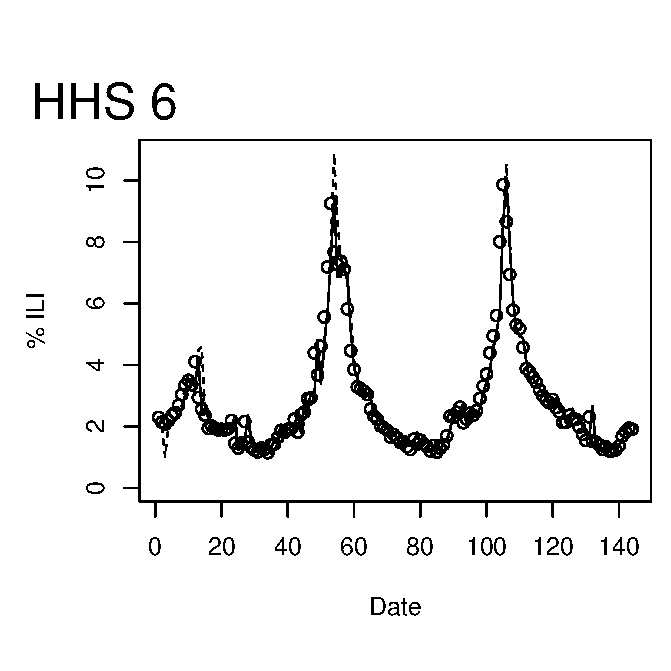
\includegraphics[width=\textwidth]{longitude/figs/nowcastHHS_6.eps}
\end{subfigure}
\end{figure}

\begin{figure}
\centering
\begin{subfigure}[b]{0.49\textwidth}
	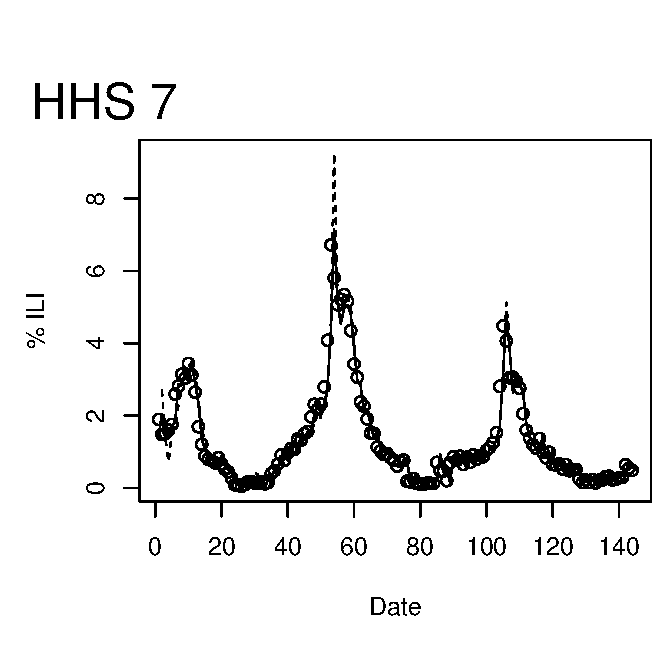
\includegraphics[width=\textwidth]{longitude/figs/nowcastHHS_7.eps}
\end{subfigure}
\begin{subfigure}[b]{0.49\textwidth}
	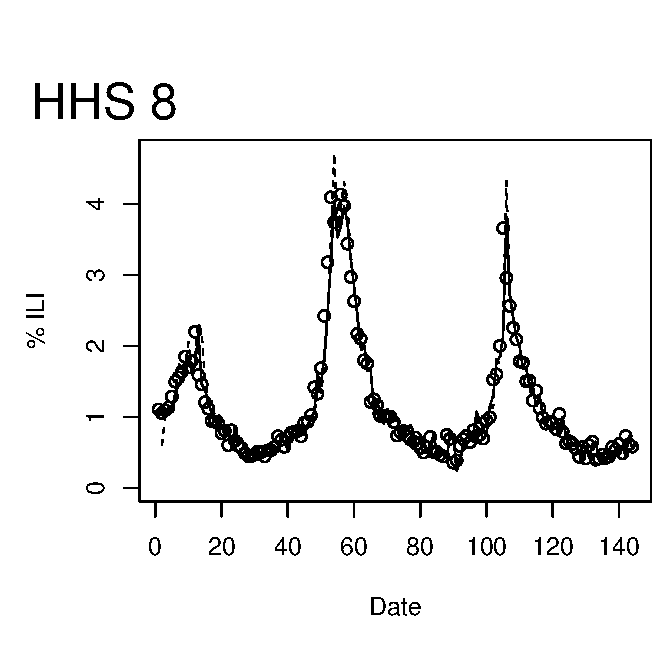
\includegraphics[width=\textwidth]{longitude/figs/nowcastHHS_8.eps}
\end{subfigure}
\\
\begin{subfigure}[b]{0.49\textwidth}
	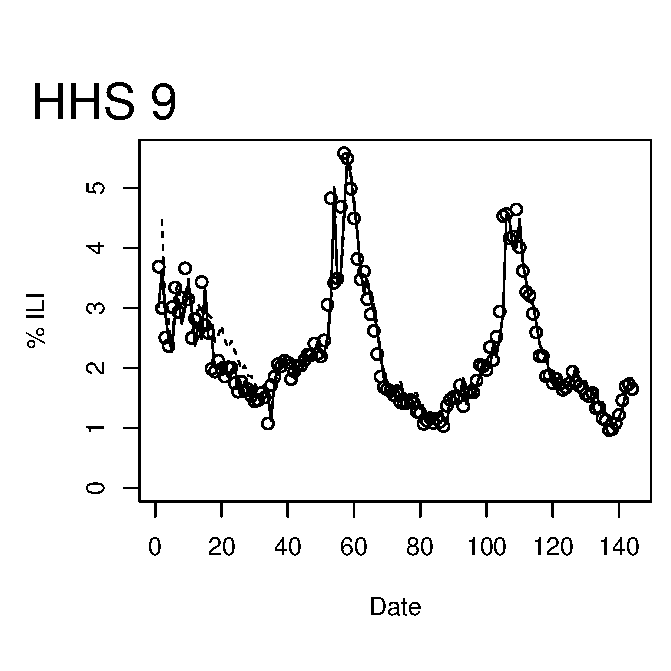
\includegraphics[width=\textwidth]{longitude/figs/nowcastHHS_9.eps}
\end{subfigure}
\begin{subfigure}[b]{0.49\textwidth}
	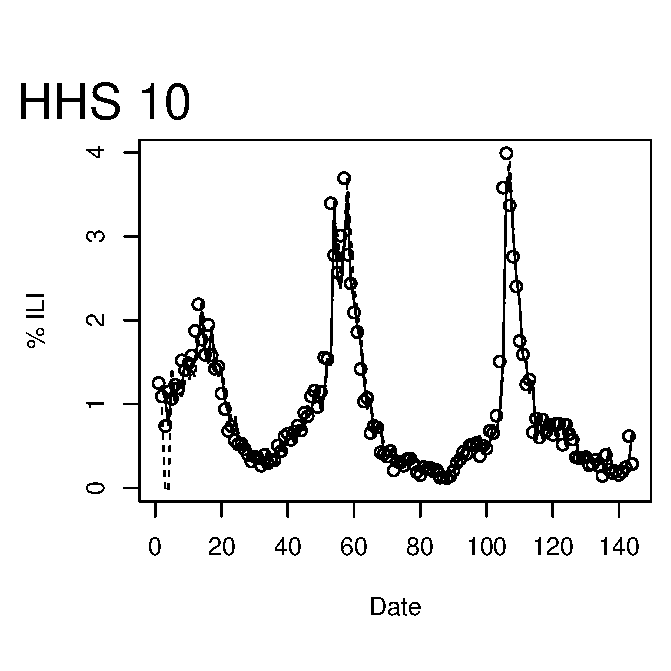
\includegraphics[width=\textwidth]{longitude/figs/nowcastHHS_10.eps}
\end{subfigure}\caption{Comparison of Twitter's forecasting (dashed lines) and retroactive measurements (solid lines) to the CDC's reported Influenza rates (circles) for each of the 10 HHS regions.}
\label{fig:hhs_curves_all}
\end{figure}


\begin{figure}
\centering
\begin{subfigure}[b]{0.49\textwidth}
	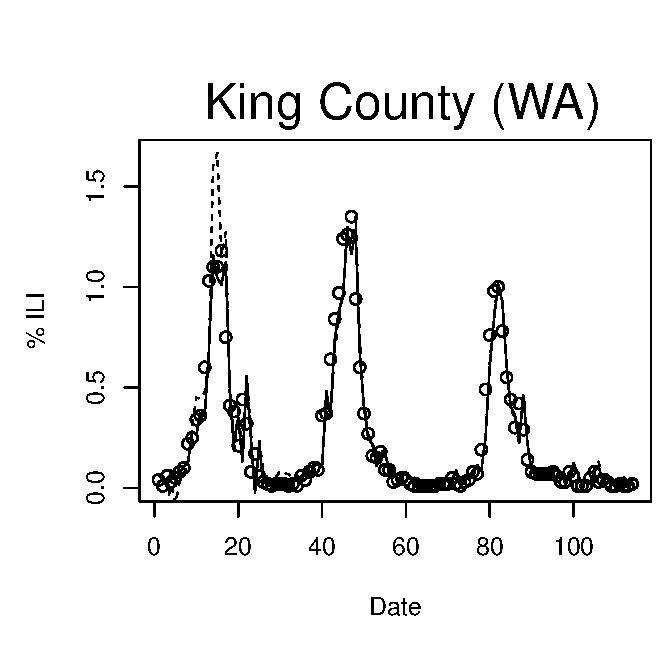
\includegraphics[width=\textwidth]{longitude/figs/nowcastLocal_seattle.eps}
\end{subfigure}
\begin{subfigure}[b]{0.49\textwidth}
	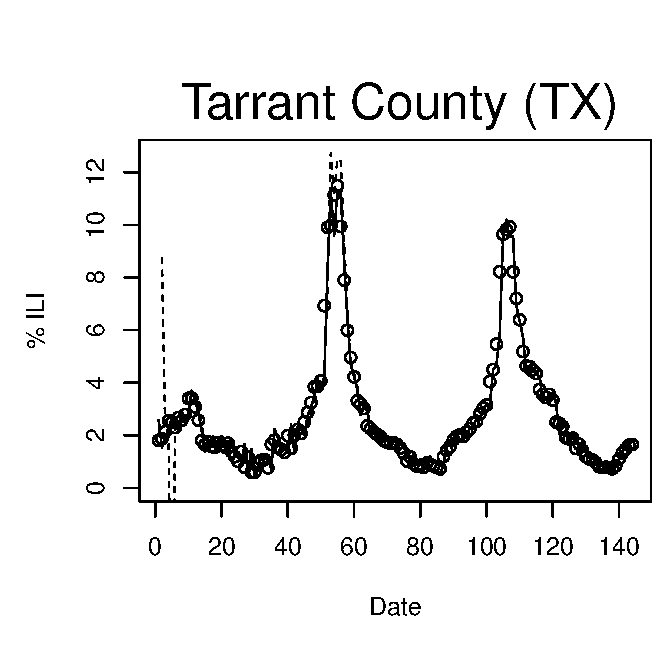
\includegraphics[width=\textwidth]{longitude/figs/nowcastLocal_texas.eps}
\end{subfigure}
\caption{Comparison of Twitter's forecasting (dashed lines) and retroactive measurements (solid lines) to the CDC's reported Influenza rates (circles) for King County and Tarrant County.}
\label{fig:local_curves_all}
\end{figure}